\documentclass[11pt, a4paper, DIV=11]{scrartcl}
\usepackage[english]{babel}
\usepackage[nolist]{acronym}
\usepackage{todonotes}
\usepackage{listings}
\usepackage{graphicx}
\usepackage[pdfborder=0]{hyperref}

\usepackage[utf8]{luainputenc}
\usepackage{luatextra} % loads fontspec and luacode, luatexbase, lualib
\usepackage{luamplib}

\author{Sven Schrader \and Eric M\"uller \and Sebastian Jeltsch}
\title{BrainScales Hardware User Guide}

\begin{document}

\maketitle

Before reading this document you should familiarize your self with the
\acs{PyNN} interface \cite{pynn}.

\section{Getting your data back}
\subsection{\texttt{get\_data()}}
Data is not guaranteed to be correct before completion of the experiment.
\todo{smoother?}
Spike data won't be available before the hardware experiment completes. % real-time buffering?
% Weight data? Solution: recoder functionality in Projection in PyNN 0.8?
Return only idealized data and should not be done anyway since random numbers
will be drawn on the user side instead of the cluster.
% Flattened PyNN description as "comparision" base between sim and emu
Getters are not allowed to be called between the first call to
\texttt{run()} and \texttt{end()} (and will throw an exception in this case).

\subsection{\texttt{record()}}
recorders yield actual results, but data is only available after
\texttt{end()}. Recordings of e.g. weights at $t=0$ reflect the actual weights
mapped to hardware.


\section{Multiple calls to \texttt{run()}}

\subsection{Incremental Experiments -- recording timeslices of data}
\begin{lstlisting}[language=Python]
for i in range(10):
    pynn.run(100.)
    # recording 10 ms of spike data...
    pop0.record('spikes')
    pynn.run(10.)
    pop0.record(None)
# t == 1100 ms
\end{lstlisting}

\subsection{Multiple Experiments -- e.g.\ sweeps}
\begin{lstlisting}[language=Python]
mapper.setLazyRun(True) # don't trigger mapping via pynn.run()
mapper.sweepHint(pps) # hint for mapping process
for ps in pps.iter_inner():
     pynn.reset()
     p0.set(ps.pp0)
     p1.set(ps.pp1)
     pynn.run(100.)
mapper.flush() # run mapping job
pynn.end() # block until experiment completes
 \end{lstlisting}

\begin{figure}[h]
    \begin{center}
        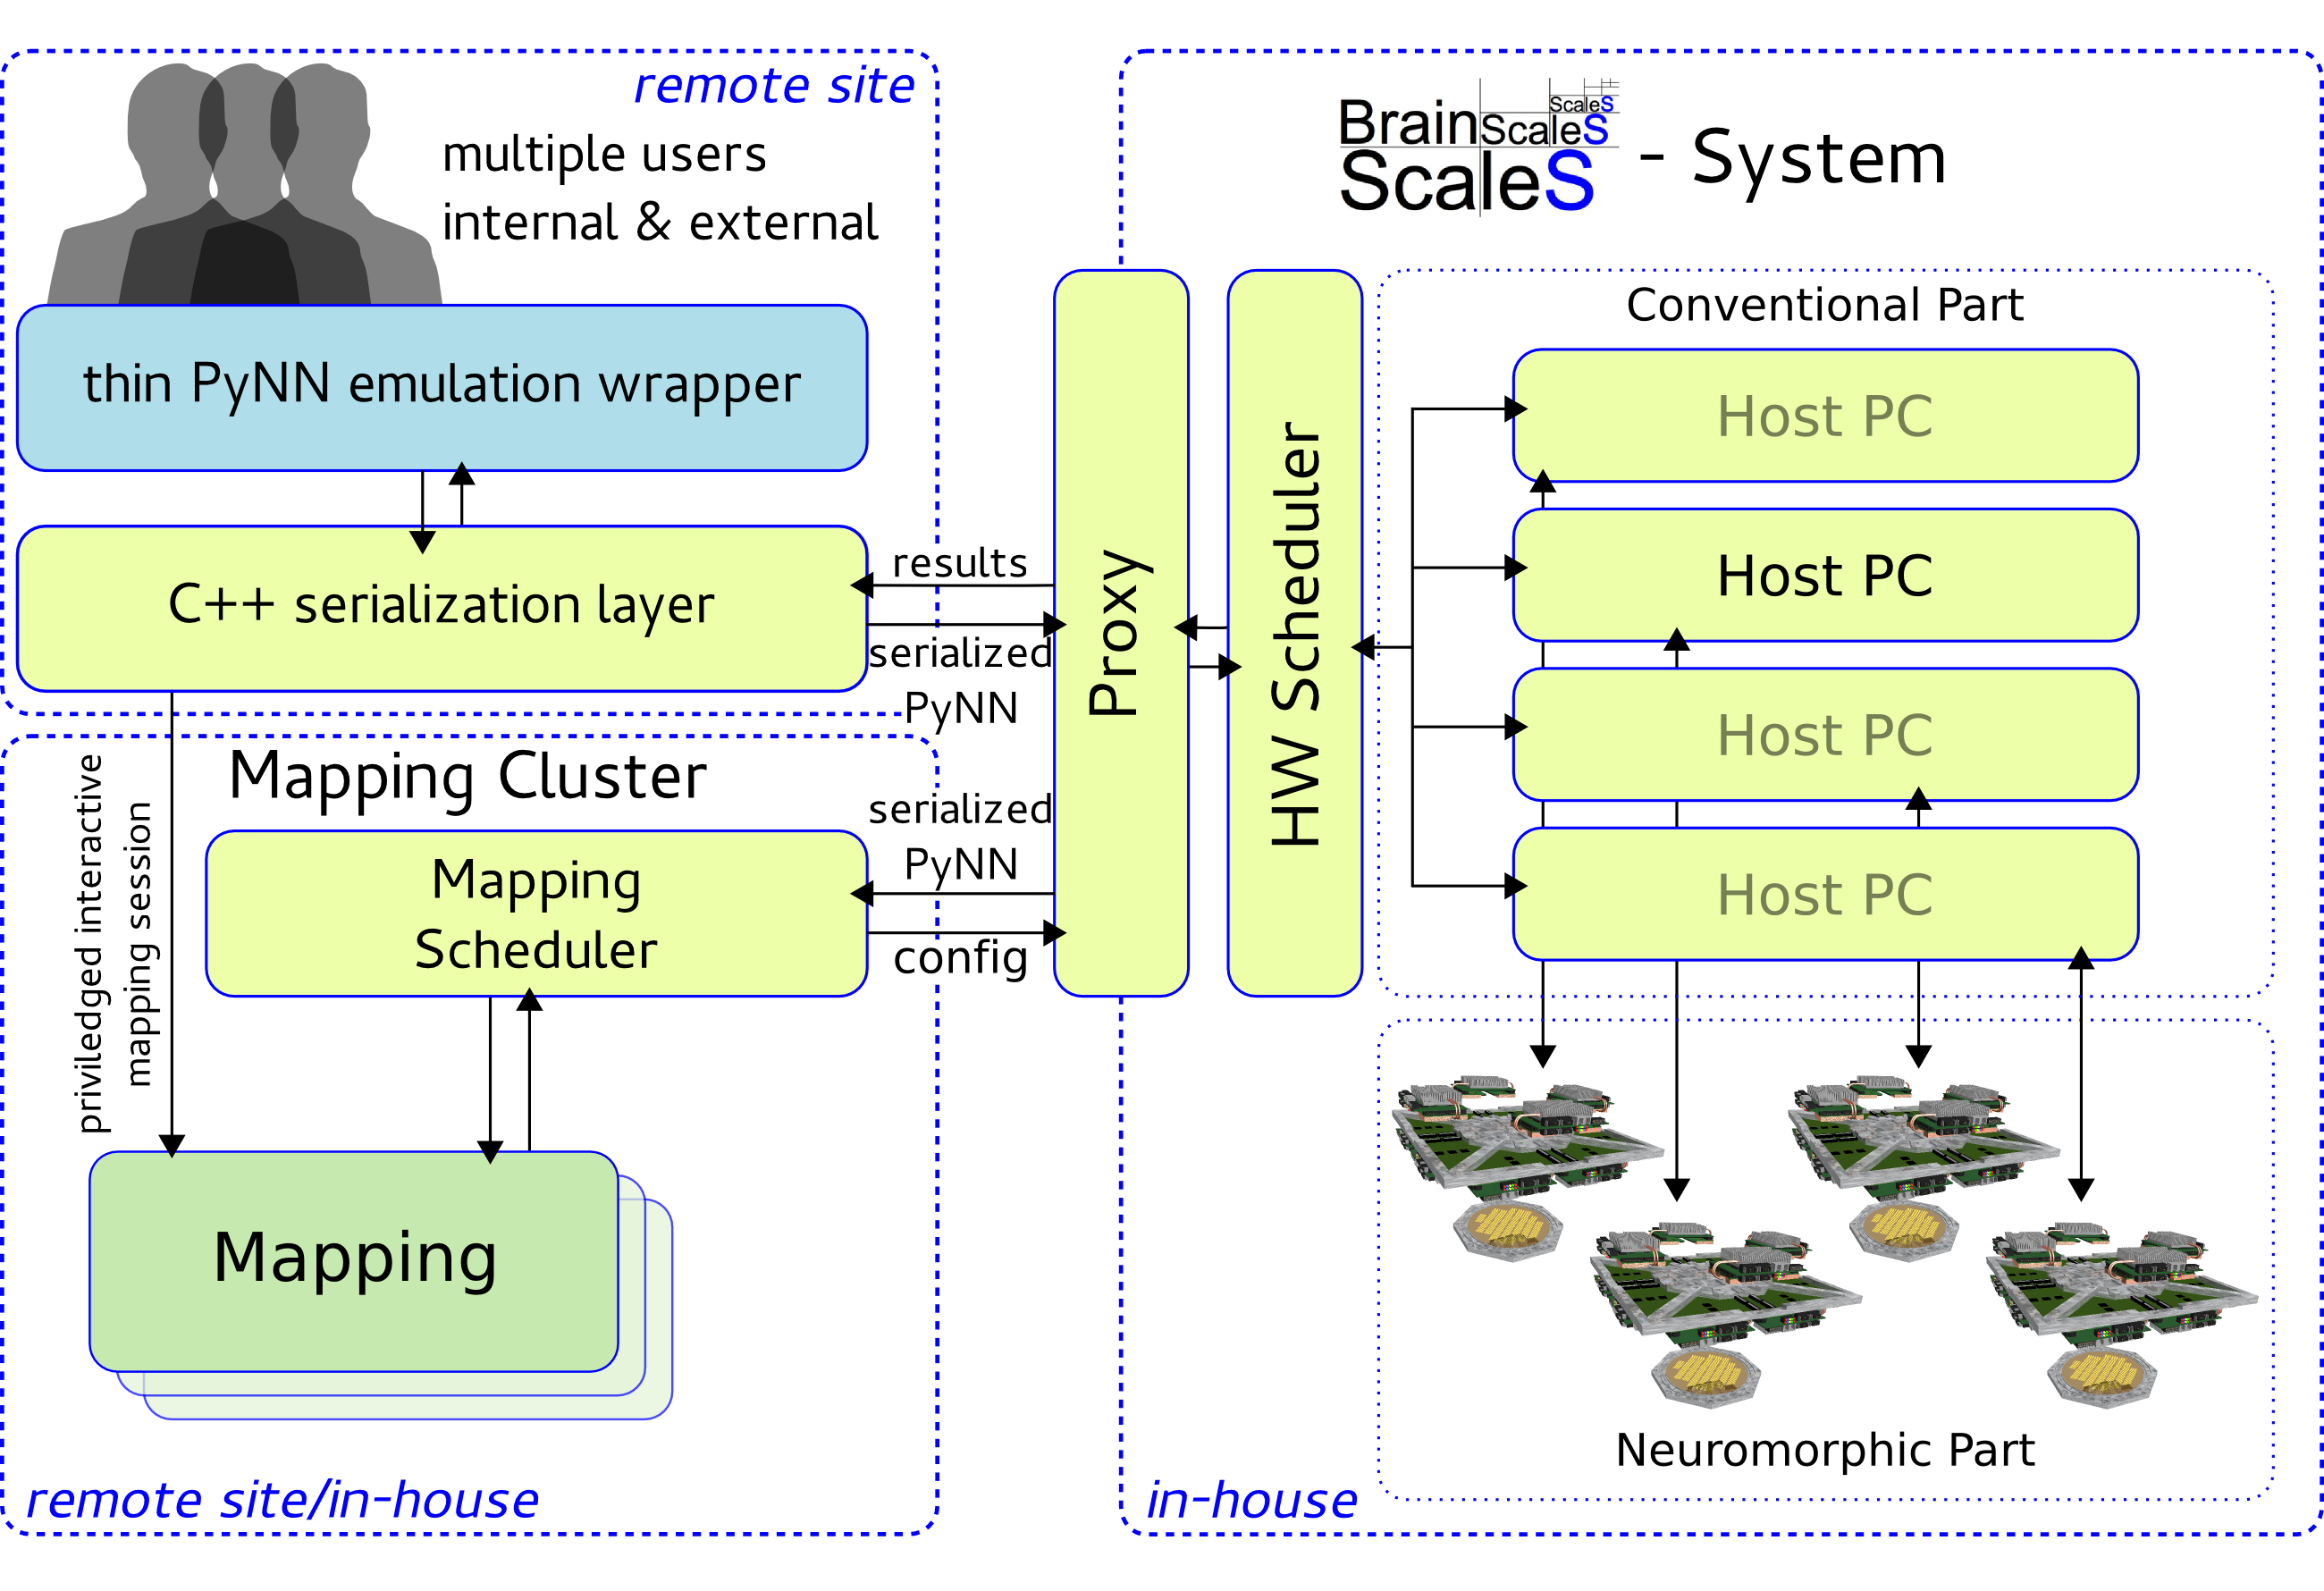
\includegraphics[width=\textwidth]{fig/flow.png}
    \end{center}
    \caption{flow}
    \label{fig:flow}
\end{figure}

%\bibliographystyle{unsrt}
%\bibliography{}

\begin{acronym}
\end{acronym}

\end{document}
